\section{Profiling and Benchmarking}
\makesubcontentsslides


%%% The need for profiling
\subsection{Why Profile?}
\makesubcontentsslidessec

\begin{frame}
  \begin{block}{Why Profile?}
  \begin{itemize}
    \item Because performance matters.
    \item Bad practices scale up!
    \item Your bottlenecks may surprise you.
    \item Because R is dumb.
  \end{itemize}
  \end{block}
\end{frame}


\begin{frame}[fragile]{Compilers often correct bad behavior\dots}
  \begin{center}
\begin{minipage}{.4\textwidth}
\vspace{0pt}
\begin{lstlisting}[title=A Really Dumb Loop,language=Rcpp]
int main(){
    int x, i;
    for (i=0; i<10; i++)
        x = 1;
    return 0;
}
\end{lstlisting}
\begin{lstlisting}[language=shl,title=clang -O3 example.c]
main:
        .cfi_startproc
# BB#0:
        xorl    %eax, %eax
        ret
\end{lstlisting}
\end{minipage}
\begin{minipage}{.57\textwidth}
\begin{lstlisting}[language=shl,title=clang example.c]
main:
        .cfi_startproc
# BB#0:
        movl    $0, -4(%rsp)
        movl    $0, -12(%rsp)
.LBB0_1:
        cmpl    $10, -12(%rsp)
        jge     .LBB0_4
# BB#2:
        movl    $1, -8(%rsp)
# BB#3:
        movl    -12(%rsp), %eax
        addl    $1, %eax
        movl    %eax, -12(%rsp)
        jmp     .LBB0_1
.LBB0_4:
        movl    $0, %eax
        ret
\end{lstlisting}
\end{minipage}

  \end{center}
\end{frame}



\begin{frame}[fragile]{R will not!}
    \begin{center}
\begin{minipage}[t]{.45\textwidth}
\begin{lstlisting}[title=Dumb Loop,escapeinside={(*@}{@*)}]


for (i in 1:n){
  Y <- (*@ \textcolor{red}{t(A)} @*) %*% Q
  Q <- qr.Q(qr(Y))
  Y <- A %*% Q
  Q <- qr.Q(qr(Y))
}

Q
\end{lstlisting}
\end{minipage}
\begin{minipage}[t]{.45\textwidth}
\begin{lstlisting}[title=Better Loop,escapeinside={(*@}{@*)}]
(*@ \textcolor{red}{tA <- t(A)} @*)

for (i in 1:n){
  Y <- tA %*% Q
  Q <- qr.Q(qr(Y))
  Y <- A %*% Q
  Q <- qr.Q(qr(Y))
}

Q
\end{lstlisting}
\end{minipage}
\end{center}
\end{frame}


\begin{frame}[fragile]{Example from a Real R Package}
    \begin{center}
\begin{minipage}[t]{.6\textwidth}
\vspace{-.9cm}
\begin{lstlisting}[title=Exerpt from Original function,escapeinside={(*@}{@*)}]
while(i<=N){
  for(j in 1:i){
    (*@ \textcolor{red}{d.k <- as.matrix(x)[l==j,l==j]}@*)
      ...
\end{lstlisting}
\vspace{-.3cm}
\begin{lstlisting}[title=Exerpt from Modified function,escapeinside={(*@}{@*)}]
(*@\textcolor{red}{x.mat <- as.matrix(x)}@*)

while(i<=N){
  for(j in 1:i){
    (*@ \textcolor{red}{d.k <- x.mat[l==j,l==j]}
@*)
      ...
\end{lstlisting}
\end{minipage}
\begin{minipage}[t]{.34\textwidth}
\vspace{1.1cm}
By changing just 1 line of code, performance of the main
method improved by \textbf{over 3.5$\times$} !
\end{minipage}
\end{center}
\end{frame}


\begin{frame}
  \begin{block}{Some Thoughts}
    \begin{itemize}
      \item R is slow.
      \item Bad programs are slower.
      \item High-level language: one line can touch a lot of data
      \item R will not fix bad programming
    \end{itemize}
  \end{block}
\end{frame}

\subsection{How to Profile and Benchmark}
\makesubcontentsslidessec

%%% Basic profiling
\begin{frame}[fragile]
  \begin{block}{Performance Profiling Tools: \code{system.time()}}
  \code{system.time()} is a basic R utility for timing expressions
\begin{lstlisting}[language=R]
x <- matrix(rnorm(20000*750), nrow=20000, ncol=750)

system.time(t(x) %*% x)
#    user  system elapsed 
#   2.187   0.032   2.324

system.time(crossprod(x))
#    user  system elapsed 
#   1.009   0.003   1.019 

system.time(cov(x))
#    user  system elapsed 
#   6.264   0.026   6.338 
\end{lstlisting}
  \end{block}
\end{frame}



\begin{frame}[fragile]
\begin{block}{Performance Profiling Tools: \code{Rprof()}}
\code{Rprof()} times the execution of all \R functions:
  \vspace{-.4cm}
\begin{lstlisting}[language=Rinteractive]
Rprof(filename="Rprof.out", append=FALSE, interval=0.02,
  memory.profiling=FALSE, gc.profiling=FALSE, 
  line.profiling=FALSE, numfiles=100L, bufsize=10000L)
\end{lstlisting}

\begin{lstlisting}[language=R]
x <- matrix(rnorm(10000*250), nrow=10000, ncol=250)

Rprof()
invisible(prcomp(x))
Rprof(NULL)

summaryRprof()

Rprof(interval=.99)
invisible(prcomp(x))
Rprof(NULL)

summaryRprof()
\end{lstlisting}
\end{block}
\end{frame}



\begin{frame}[fragile,shrink]
  \begin{block}{Performance Profiling Tools: \code{Rprof()}}
  \vspace{-.5cm}
\begin{lstlisting}[language=R]
$by.self
                self.time self.pct total.time total.pct
"La.svd"             0.68    69.39       0.72     73.47
"%*%"                0.12    12.24       0.12     12.24
"aperm.default"      0.04     4.08       0.04      4.08
"array"              0.04     4.08       0.04      4.08
"matrix"             0.04     4.08       0.04      4.08
"sweep"              0.02     2.04       0.10     10.20
### output truncated by presenter

$by.total
                 total.time total.pct self.time self.pct
"prcomp"               0.98    100.00      0.00     0.00
"prcomp.default"       0.98    100.00      0.00     0.00
"svd"                  0.76     77.55      0.00     0.00
"La.svd"               0.72     73.47      0.68    69.39
### output truncated by presenter

$sample.interval
[1] 0.02

$sampling.time
[1] 0.98
\end{lstlisting}
  \end{block}
\end{frame}



\begin{frame}[fragile]
  \begin{block}{Performance Profiling Tools: \code{Rprof()}}
  \vspace{-.5cm}
\begin{lstlisting}[language=R]
$by.self
[1] self.time  self.pct   total.time total.pct 
<0 rows> (or 0-length row.names)

$by.total
[1] total.time total.pct  self.time  self.pct  
<0 rows> (or 0-length row.names)

$sample.interval
[1] 0.99

$sampling.time
[1] 0
\end{lstlisting}
  \end{block}
\end{frame}



\begin{frame}[fragile]
  \begin{block}{Performance Profiling Tools: rbenchmark}
  \pkg{rbenchmark} is a simple package that easily benchmarks different 
functions:
\begin{lstlisting}[language=R]
x <- matrix(rnorm(10000*500), nrow=10000, ncol=500)

f <- function(x) t(x) %*% x
g <- function(x) crossprod(x)

library(rbenchmark)
benchmark(f(x), g(x))

#   test replications elapsed relative
# 1 f(x)          100  64.153    2.063
# 2 g(x)          100  31.098    1.000
\end{lstlisting}
  \end{block}
\end{frame}



%%% Advanced profiling
%\subsection{Advanced R Profiling}
\makesubcontentsslidessec

\begin{frame}
  \begin{block}{Other Profiling Tools}
    \begin{itemize}
      \item perf (Linux)
      \item PAPI
      \item MPI profiling: fpmpi, mpiP, TAU
    \end{itemize}
  \end{block}
\end{frame}


\begin{frame}[fragile]
  \begin{block}{Profiling MPI Codes with \textbf{pbdPROF}}
  \begin{minipage}[t]{.58\textwidth}
  \vspace{.2cm}
  \vspace{0pt}
  1. Rebuild \pbdR\ packages
\vspace*{-.5cm}
\begin{lstlisting}[language=shl,title=\ ]
R CMD INSTALL pbdMPI_0.2-1.tar.gz \ --configure-args= \ "--enable-pbdPROF"
\end{lstlisting}
2. Run code
\vspace*{-.5cm}
\begin{lstlisting}[language=shl,title=\ ]
mpirun -np 64 Rscript my_script.R
\end{lstlisting}

3. Analyze results
\vspace{-.5cm}
\begin{lstlisting}[title=\ ]
library(pbdPROF)
prof <- read.prof( "output.mpiP")
plot(prof, plot.type="messages2")
\end{lstlisting}

  \end{minipage}
  \hfill
  \begin{minipage}[t]{.4\textwidth}
  \vspace{0pt}
    \centering
    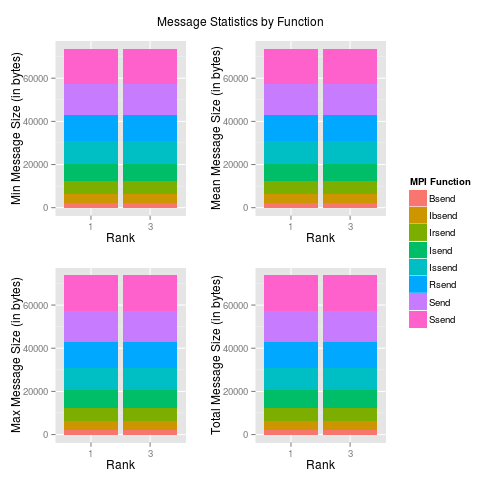
\includegraphics[scale=.25]{../common/pics/mpip}
    \\[.1cm]
    
\includegraphics[scale=0.35]{../common/pics/gsoc}
  \end{minipage}
  \end{block}
\end{frame}





\begin{frame}[fragile]
  \begin{block}{Profiling with \textbf{pbdPAPI}}
  \begin{minipage}{.6\textwidth}
    \begin{itemize}
      \item Performance Application Programming Interface
      \item High and low level interfaces
      \item Linux only :(
    \end{itemize}  
  \end{minipage}
  \begin{minipage}{.38\textwidth}
    \centering
    
\includegraphics[scale=0.12]{../common/pics/gsoc_2014}
  \end{minipage}
\begin{center}
\begin{tabular}{ll} \hline\hline
Function & Description of Measurement \\ \hline
\code{system.flips()} & Time, floating point instructions, and Mflips \\
\code{system.flops()} & Time, floating point operations, and Mflops \\
\code{system.cache()} & Cache misses, hits, accesses, and reads \\
\code{system.epc()} & Events per cycle \\
\code{system.idle()} & Idle cycles \\
\code{system.cpuormem()} & CPU or RAM bound$^*$ \\
\code{system.utilization()} & CPU utilization$^*$ \\
\hline\hline
\end{tabular}
\end{center}
  \end{block}
\end{frame}


\subsection{Summary}
\makesubcontentsslidessec


\begin{frame}[fragile]
  \begin{block}{Summary}\pause
    \begin{itemize}
      \item Start by loading the package:
\vspace{-.4cm}
\begin{lstlisting}
library(pbdMPI, quiet = TRUE)
\end{lstlisting}
      \item Always initialize before starting and finalize when finished:
\vspace{-.4cm}
\begin{lstlisting}
init()

# ...

finalize()
\end{lstlisting}
\end{itemize}
\end{block}
\end{frame}